\documentclass[11pt]{article}
\usepackage[utf8]{inputenc}
\usepackage{hyperref}
\usepackage{enumerate}
\usepackage{algorithm}
\usepackage{algpseudocode}
\usepackage{fullpage}
\usepackage{mdwlist}
\usepackage{hyperref}
\usepackage{listings}
\usepackage{color}
\usepackage{graphicx}
\graphicspath{ {.} }
\usepackage[superscript,biblabel]{cite}

\definecolor{mygreen}{rgb}{0,0.6,0}
\definecolor{mygray}{rgb}{0.5,0.5,0.5}
\definecolor{mymauve}{rgb}{0.58,0,0.82}

\lstset{ %
  backgroundcolor=\color{white},   % choose the background color; you must add \usepackage{color} or \usepackage{xcolor}
  basicstyle=\footnotesize,        % the size of the fonts that are used for the code
  breakatwhitespace=false,         % sets if automatic breaks should only happen at whitespace
  breaklines=true,                 % sets automatic line breaking
  captionpos=b,                    % sets the caption-position to bottom
  commentstyle=\color{mygreen},    % comment style
  deletekeywords={...},            % if you want to delete keywords from the given language
  escapeinside={\%*}{*)},          % if you want to add LaTeX within your code
  extendedchars=true,              % lets you use non-ASCII characters; for 8-bits encodings only, does not work with UTF-8
  frame=single,                    % adds a frame around the code
  keepspaces=true,                 % keeps spaces in text, useful for keeping indentation of code (possibly needs columns=flexible)
  keywordstyle=\color{blue},       % keyword style
  language=Lisp,                 % the language of the code
  otherkeywords={*,...},            % if you want to add more keywords to the set
  numbers=left,                    % where to put the line-numbers; possible values are (none, left, right)
  numbersep=5pt,                   % how far the line-numbers are from the code
  numberstyle=\tiny\color{mygray}, % the style that is used for the line-numbers
  rulecolor=\color{black},         % if not set, the frame-color may be changed on line-breaks within not-black text (e.g. comments (green here))
  showspaces=false,                % show spaces everywhere adding particular underscores; it overrides 'showstringspaces'
  showstringspaces=false,          % underline spaces within strings only
  showtabs=false,                  % show tabs within strings adding particular underscores
  stepnumber=1,                    % the step between two line-numbers. If it's 1, each line will be numbered
  stringstyle=\color{mymauve},     % string literal style
  tabsize=2,                       % sets default tabsize to 2 spaces
  title=\lstname                   % show the filename of files included with \lstinputlisting; also try caption instead of title
}

\begin{document}

\title{ Inspection of Lisp - Names, Bindings, Scopes and Types }
\date{March 30, 2015}
\author{Mahmut Bulut - 14501026\\ Computer Engineering Dept., Yıldız Technical University}

\maketitle
\paragraph{Naming in Lisp} ~\\

\par
In Lisp symbols are just a name. Naming makes new relations internally. Symbols are  datatypes in Lisp. Also symbols are unique identifiers that are identical to other symbols with the same name without restricton with case-sensitivity.
\par
On the other hand Lisp also names functions as variables. This is a distinction with other programming languages.
\begin{lstlisting}
=> (setq first 'the-bender)
-> THE-BENDER

=> (first (list 3 2 1))
-> 3

=> first
-> THE-BENDER
\end{lstlisting}
At first and the last one \textit{first} is used as variable. But at second first is used as function.
In Lisp a value can more than one name. This makes aliasing easy and useful.\footnote{\url{http://psg.com/~dlamkins/sl/chapter03-05.html}}

\paragraph{Binding in Lisp} ~\\

\par
Lisp has lexical binding which means that a variable declared with \textit{let} statement will be lexically bound at compile time and cannot be reach outside of lexical scope of \textit{let}.\footnote{\url{https://www.gnu.org/software/emacs/manual/html_node/elisp/Lexical-Binding.html}} In other words this can be called as static binding.

\begin{lstlisting}
(let ((data 1))    ; data is lexically bound.
  (+ data 3))
=> 4

(defun getdata ()
  data)            ; data is used free in this function.

(let ((data 1))    ; data is lexically bound.
  (getdata))
;error--> Symbol's value as variable is void: data
\end{lstlisting}

In addition to lexical binding there is also dynamic binding. In dynamic binding variables lives in one global namespace and can be accessed amongst each other. \footnote{\url{http://emacswiki.org/emacs/DynamicBindingVsLexicalBinding\#toc2}} Dynamic binding makes easier to code greater programs with ease but decrease security with all open namespace, symbol and variable definitions.

\paragraph{Scope in Lisp} ~\\

There are several ways to determine the scope:
\begin{itemize}
\item
Place of the reference in the expression.
\item
Kind of reference translation takes place.
\item
Location of reference
\item
Declaring a variable in local or global scope
\item
Environment which solves variable bindings within its context.
\end{itemize}
There are three types of environment in Lisp\footnote{\url{http://en.wikipedia.org/wiki/Common_Lisp\#Kinds_of_environment}}; global, dynamic and lexical.
\textbf{Global} environment is like its name global across a program if a declaration made in it, it will be known through the program.
\textbf{Dynamic} environment is generator like environment. It binds at constructive expressions like \textit{let} block.
\textbf{Lexical} environment defines a lexical scope within a expression and scope will last as long as this expression lasts.

\paragraph{Types in Lisp} ~\\

\par
Data types are generally set of Lisp objects. But lisp has two main types:
\begin{itemize}
\item atom
\item list
\end{itemize}
Lists contains atoms or lists of elements. Atoms are seperated in lists from each other with whitespace and they cannot contain anything else except itself\footnote{\url{http://graham.main.nc.us/~bhammel/graham/lisp.html}}. With this seperation expression can be made with combination of lists ad atoms\footnote{\url{https://www.gnu.org/software/emacs/manual/html_node/eintr/Lisp-Atoms.html}}. These types can be included in global scope and it makes easier to infer or coerce between each other. There is already a function named \textbf{coerce} in Comman Lisp.\footnote{\url{https://www.cs.cmu.edu/Groups/AI/html/cltl/clm/node52.html}}
In addition to it empty data type, which contains no data object are defined by \textit{nil} type.
Every type can be created from its relative types and coerce with them. You can see Common Lisp type hierarchy in Fig. 1.~\ref{fig:clisphier}


\begin{figure}
\label{fig:clisphier}
\caption{Common Lisp Type Hierarchy}
\centering
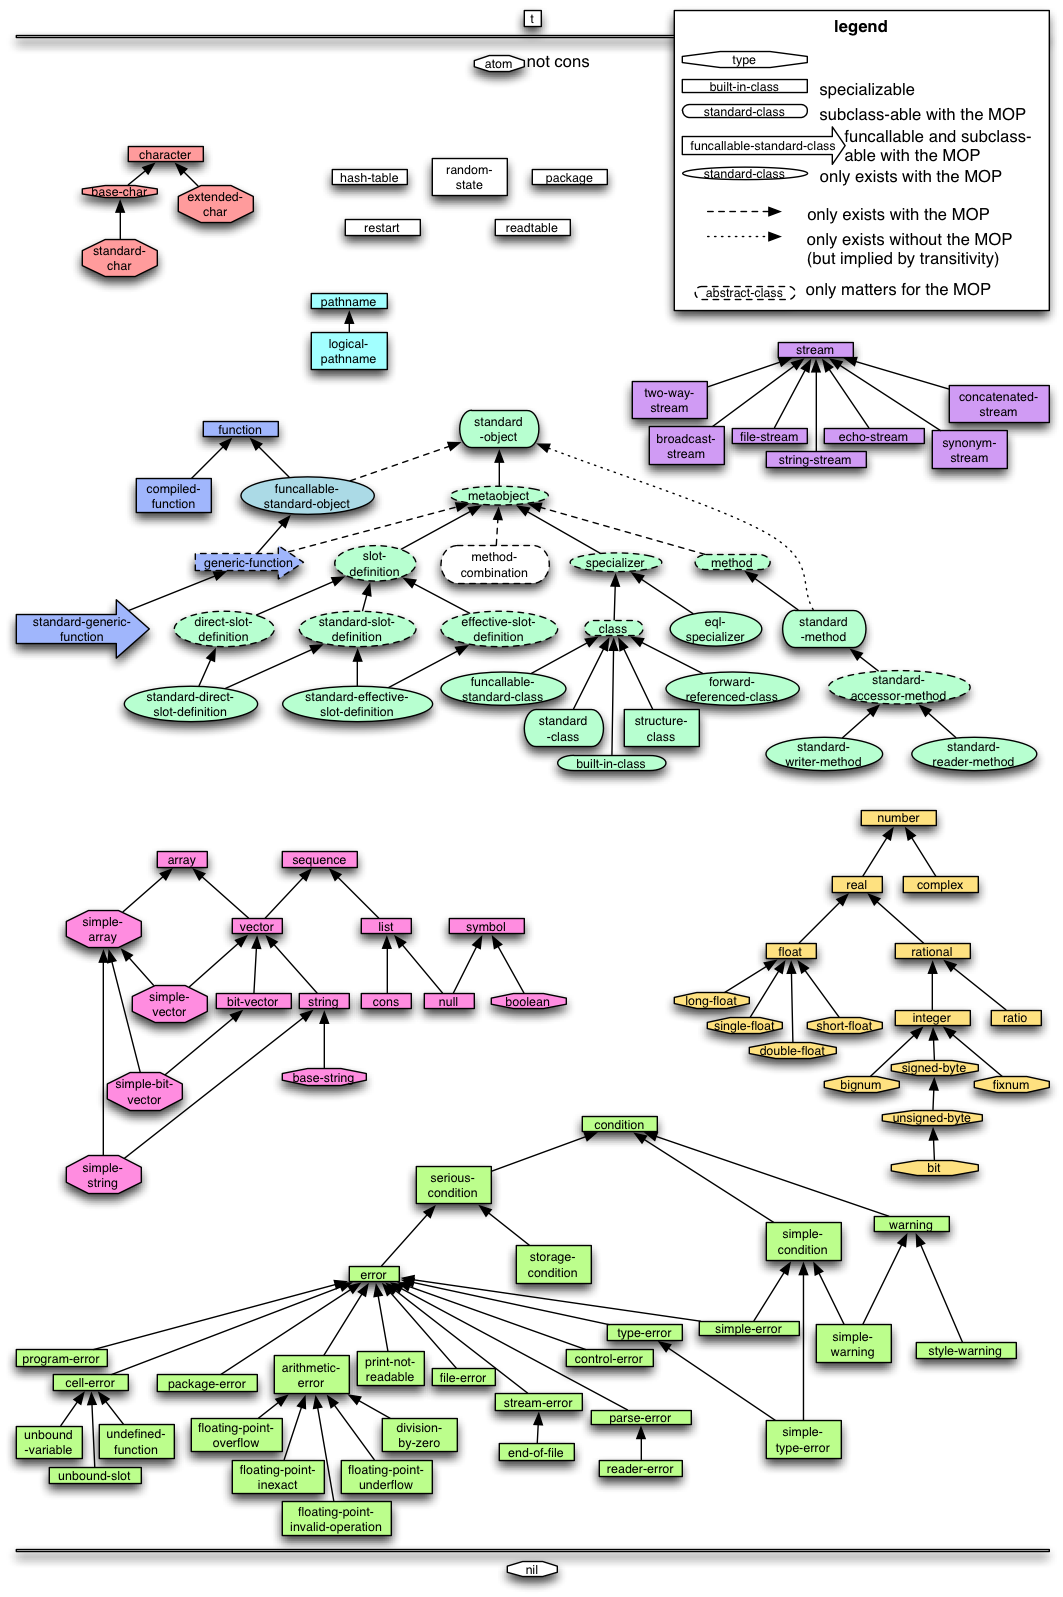
\includegraphics[width=0.85\textwidth]{CL-type-hierarchy}
\end{figure}

\listoffigures

\end{document}
